\documentclass[a4paper, 10pt, pdftex]{report}
  \usepackage[dutch]{babel}
  \usepackage{ulem}
  \usepackage{alltt}
  \usepackage{amssymb}

  %graphics
  \usepackage{graphicx}
  \usepackage{wrapfig}

  %links
  \usepackage{hyperref}
  \usepackage[all]{hypcap}

  %colours
  \usepackage[table]{xcolor}
  \definecolor{lightgray}{gray}{0.90}

  %references
  \usepackage{natbib}
  \bibpunct{(}{)}{;}{a}{,}{,}

  % metadata
  \title{\textsc{Participatie op learning networks verhogen door middel van gebruiksvriendelijkheid} \linebreak (werktitel) \linebreak \emph{Projectverslag}}
  \author{\textbf{Kilian Valkhof}\\
  Hogeschool Rotterdam\\
  \textit{studentnr.:} 0783312\\
  \\
  \textit{Afstudeerbegeleider:} Sandra Hekkelman\\
  \textit{Tweede begeleider:}\\
  \\
  \textit{Bedrijf:} Wakoopa bv.\\
  \textit{Bedrijfsbegeleider:} Robert Gaal}

  \date{17 augustus 2009 -- \today}

  \makeindex


  %prettypage
  %\hoffset = -0.6in
  %\textwidth = 6in

  \usepackage{lastpage}
  \usepackage{fancyhdr}
  \pagestyle{fancy}
  \fancyhead{}
  \fancyfoot{}

  \lhead{}
  \rhead{}
  \lfoot{$Projectverslag$}
  \rfoot{\thepage~van \pageref*{LastPage}}
  \renewcommand{\headrulewidth}{0.0pt}
  \renewcommand{\footrulewidth}{0.4pt}

  % List items
  \renewcommand{\theenumi}{\roman{enumi}}
  \renewcommand{\labelenumi}{\theenumi}
  \renewcommand{\theenumii}{\alph{enumii}}
  \renewcommand{\labelenumii}{\theenumii}

\begin{document}
  \normalem
  \maketitle

  \newpage
  \chapter*{Samenvatting}
  \addcontentsline{toc}{chapter}{Samenvatting}

  \newpage
  \tableofcontents

  \newpage
  \section*{Introductie}
  \addcontentsline{toc}{chapter}{Introductie}
    In de recente jaren zijn er een tweetal dingen gebeurd: sociale netwerken hebben een explosieve groei doorgemaakt
  en gebruiksvriendelijkheid voor websites hebben (terecht) een veel grotere nadruk gekregen dan daarvoor. Hoewel mensen
  als Jacob Nielsen en Jesse James Garrett het ons al jaren vertellen, is het pas de afgelopen jaren `normaal' geworden
  om ook aandacht te besteden aan gebruiksvriendelijkheid. Veel van de theorie op dit gebied focust zich echter op
  informatieve websites (nieuwssites, bedrijfswebsites en weblogs) en minder op de nieuwe vorm van websites: learning networks.

    Een sociaal netwerk staat of valt bij participatie van haar gebruikers. Omdat de interactiviteit van dit soort websites zo'n grote rol speelt, is het belangrijk dat de gebruiker zo min mogelijk drempels tegen komt tijdens het gebruiken van de website. Het weghalen van drempels wordt gebruiksvriendelijkheid genoemd. Dit verslag richt zich op deze gebruiksvriendelijkheid met als doel de interactiviteit beter te laten verlopen en zo de participatie op het sociale netwerk te verhogen.

  Doordat mensen op sociale netwerken heel anders bezig zijn dan op gewone informatieve websites --- er sprake van interactie in plaats van passief lezen --- Denk ik dat dit gevolgen heeft voor de gebruiksvriendelijkheid. Waar gebruiksvriendelijkheid op informatieve websites gaat om het effectief vinden van informatie, is het hoofddoel van sociale netwerken de participatie. Mijn afstudeerbedrijf, \emph{Wakoopa}, is zo'n sociaal netwerk, en is daarom met mij geinteresseerd in het verbeteren van de gebruikersvriendelijkheid van de website en het uitvinden welke factoren voor meer participatie zorgen.

    Gedurende mijn minor user experience design heb ik veel aandacht besteed aan gebruiksvriendelijkheid en hoe de gebruiksvriendelijkheid van design goed vertaalt kan worden naar werkende code. Ik hoop dit door te kunnen zetten bij Wakoopa gedurende mijn afstudeertraject.




    \section{Introductie van Wakoopa}
      Een korte introductie van Wakoopa is voor het verdere verslag van belang, zodat de lezer een duidelijk beeld heeft van Wakoopa als learning network en de mogelijkheden daarvan. Op de About pagina van Wakoopa \citep{Gaal2007} staat de volgende beschrijving:
        \begin{quote} Wakoopa is a learning network that helps people discover the best software, games and web apps on the market. Sign-up, install a small tracker on your desktop and automatically create your online software profile that you can share with friends and the world, also through widgets. Wakoopa keeps you updated about what your contacts are using, and sends you smart recommendations. Games, audio \& video players, instant messengers or office tools: Wakoopa knows what's hot.
        \end{quote}
      Door het installeren van een kleine applicatie op je computer (de tracker), kan Wakoopa bijhouden welke applicaties je allemaal op je computer gebruikt. Deze gegevens worden in een online profiel weergegeven. Daarnaast kunnen gebruikers hun mening geven over de applicaties die zij gebruiken. Dit wordt gecombineerd met een sociaal aspect van het leggen van contacten, het maken van teams, het behalen van punten en het \emph{raten} van applicaties.

        \subsection{Wakoopa als learning network}
        In hun paper \emph{Functionality for learning networks: lessons learned from social web application} noemen \citeauthor{Berlanga2007} een aantal kenmerken van sociale netwerken die ook \emph{learning networks} zijn. In plaats van het maken van contacten is het focuspunt van deze sociale netwerken objecten. Een voorbeeld hiervan is Flickr, een sociaal network rondom foto's. Op Wakoopa zijn deze objecten de applicaties die je gebruikt. Om vast te stellen of Wakoopa onder dezelfde categorie valt en om een overzicht te geven van de functionaliteit die Wakoopa biedt, zullen we in tabellen \ref{tab:functies} \ref{tab:acties} en \ref{tab:metaacties} \label{learningnetwork} Wakoopa vergelijken met de kenmerken die \citeauthor{Berlanga2007} hebben opgesteld.

         De drie door \citeauthor{Berlanga2007}  onderzochte learning networks (Delicious, Youtube en Flickr) bevatten niet \emph{alle} omschreven functionaliteit, maar worden hoe dan ook als \emph{learning networks} omschreven. Wakoopa voldoet in deze tabellen ook niet aan alle vereisten, maar zit qua functionaliteit op vergelijkbare hoogte met Youtube en Flickr (waarbij Delicious minder functionaliteit bied). We kunnen Wakoopa dus als learning network beschouwen.

        \begin{table}[ht]
        \centering
        \caption{Self-management functionality}
        \rowcolors{1}{white}{lightgray}
        \begin{tabular}{r|l}
          × & Wakoopa \\ \hline
          Profile & \checkmark \\
          Contacts & \checkmark \\
          Resources & \\
          Tagging & \checkmark
        \end{tabular}
        \label{tab:functies}
        \end{table}
        \begin{table}[ht]
        \centering
        \caption{Self-organisation functionality}
        \rowcolors{1}{white}{lightgray}
        \begin{tabular}{r|l}
          × & Wakoopa \\ \hline
          Comment & \checkmark \\
          Recommend & \\
          Copy & \\
          Subscribe & \checkmark \\
          Add as favourite & \checkmark \\
          Rate & \checkmark \\
          Related resources & \checkmark \\
          Search & Software, Users, Teams, Developers
        \end{tabular}
        \label{tab:acties}
        \end{table}
        \begin{table}[ht]
        \centering
        \caption{Self-regulation functionality}
        \rowcolors{1}{white}{lightgray}
        \begin{tabular}{r|l}
          Markeer\ldots & Wakoopa \\ \hline
          Resources as offensive & \checkmark \\
          Communities as offensive & \\
          Private and public resources & \checkmark \\
          Private and public communities/groups & \checkmark
        \end{tabular}
        \label{tab:metaacties}
        \end{table}


  \newpage
  \section*{Voorwoord}
  \addcontentsline{toc}{chapter}{Voorwoord}

  \newpage
  \section*{Doelstelling}
  \addcontentsline{toc}{chapter}{Doelstelling}
    Het doel van deze afstudeerstage is uitvinden welke usability factoren invloed hebben op de participatie van gebruikers van sociale netwerken. Ik hoop met een set aanbevelingen te kunnen komen die specifiek gericht zijn op sociale netwerken, en deze aanbevelingen op de site van Wakoopa door te kunnen voeren als casus. Via deze methode kan ik zeggen of de factoren inderdaad invloed hebben, en in welke mate.

  \section*{Probleemstelling}
  \addcontentsline{toc}{chapter}{Probleemstelling}
    Deze afstudeerstage heeft de volgende onderzoeksvraag:
    \begin{quotation}
     \textbf{Hoe kan de participatie op een learning network verhoogd worden door middel van usability?}
    \end{quotation}

  \section*{Afbakening van onderzoek}
  \addcontentsline{toc}{chapter}{Afbakening van onderzoek}
    Voor dit onderzoek stellen we twee afbakeningen. Ten eerste onderzoeken we niet alle sociale netwerken, maar kijken enkel naar learning networks zoals uitgelegd in de vorige sectie. Dit doen we omdat de interactie op Learning networks zoals Wakoopa of Flickr anders is dan die van bijvoorbeeld Hyves of Facebook. Deze twee laatste hebben als hoofddoel je in contact te houden met vrienden. Op learning networks is dit ook mogelijk, maar de focus van de interactie (en daarmee de gebruikersdoelen) ligt expliciet op de objecten waaromheen het netwerk is opgebouwd (zoals software of foto's). Vanwege deze focus is het niet mogelijk bevindingen direct op sociale netwerken in het algemeen toe te passen.

    Binnen deze afbakening van learning networks stellen we een tweede afbakening. Voor het analyseren gebruiken we gegevens en informatie van Wakoopa, omdat we toegang hebben tot statistieken en enqueteringsdata en de mogelijkheid hebben om A/B testing uit te voeren. Met deze opties kunnen we een holistisch inzicht in de gebruikersvriendelijkheid van een learning network krijgen. Wat we hierdoor binnen dit project niet doen is het onderzoeken in hoeverre de bevindingen van toepassing zijn op andere sociale netwerken. Naar aanleiding van testgegevens komen we met een set van aanbevelingen die op een globaal niveau zullen werken op learning networks, maar zullen dit niet met testdata op andere sociale netwerken onderbouwen.

  \newpage
  \chapter{Wat zeggen andere onderzoeken op het gebied van usability en sociale netwerken?}
    \label{researchchapter}
    \newpage

    Dit hoofdstuk onderzoekt wat papers en andere bronnen over usability op learning networks en online communities zeggen en hoe dit tot verhoging van de participatie zorgt. Naast deze papers worden er ook drie usability reviews uitgevoerd op Wakoopa onderzocht.


    \section{Externe onderzoeken}
      \subsection{\cite{Beenen2004}}

      In \emph{Using social psychology to motivate contributions to online communities} onderzoeken \citeauthor{Beenen2004} welke factoren en stimulansen bijdragen aan meer participatie van gebruikers, in hun case die van een filmsite. Door middel van een onderzoek met doelen voor gebruikers, waarbij ze de bewoording aanpasten, kwamen ze tot de conclusie dat, wanneer je aan een gebruiker duidelijk maakt hoe uniek ze zijn, ze dan veel meer zullen participeren op de website. Daarentegen is het heel lastig ze te motiveren. Enkel het noemen van voordelen om te participeren zorgt er volgens hun onderzoek voor dat mensen dat minder snel zullen doen. Een mogelijke verklaring die ze hiervoor geven is dat, wanneer mensen vertelt wordt dat ze iets moeten doen, ze minder snel geneigd zijn dat ook daadwerkelijk te doen.

      Volgens het onderzoek werkt dit zo, omdat mensen gestimuleerd worden door intrensieke motivatie, maar juist minder snel zullen participeren wanneer ze een extrensieke motievatie wordt gegeven. De overkoepelende conclusie is dat je gebruikers moet tonen hoe uniek hun bijdragen zijn, zonder dat je daarbij vermeld wat de voordelen van deze bijdragen zijn.

     \subsection{\cite{Sohn2005}}

      In \emph{Dimensions of interactivity: Differential effects of social and psychological factors} onderzoeken \citeauthor{Sohn2005} uit welke componenten interactiviteit bestaat, en welke eigenschappen of omgevingen van invloed zijn op deze componenten. Uit hun onderzoek blijkt dat interactie bestaat uit een drietal componenten:
        \begin{enumerate}
          \item Controle
          \item Reactiekwaliteit
          \item Werkbaarheid van de interactie
        \end{enumerate}
      Na analyse van de eigenschappen van proefpersonen en hun netwerk, kwamen er vier factoren uit die invloed hadden op de componenten van interactiviteit. Deze zijn:
        \begin{description}
          \item[Need for cognition]
            Need for cognition is een term die gebruikt wordt om aan te geven hoe leergierig je bent.
          \item[Web usage time]
            De tijd die je op het web spendeert.
          \item[Communication direction]
            de richting van de communicatie, dit kan naar de proefpersoon zijn, maar de proefpersoon kan tegen met andere mensen uit zijn netwerk praten.
          \item[Network density]
            Dit is de mate waarin de sociale relaties van de proefpersoon ook connecties met elkaar hebben. Met andere woorden: hoeveel van jouw vrienden kennen anderen van jouw vrienden?
        \end{description}
        Van deze vier factoren waren \emph{need for cognition} en \emph{web usage time} de meest significante indicatoren voor de mate waarin de gebruiker interactiviteit ervaart. \emph{Need for cognition} was van importantie bij alle drie de componenten. \emph{Web usage time} enkel op de werkbaarheid van de interactie. \emph{Communition direction} en \emph{Network density} hebben beide invloed op de reactiekwaliteit.

        \paragraph{}
        Voor learning networks in het algemeen betekent dit een aantal dingen:
        \begin{itemize}
          \item Maak het gemakkelijk om connecties met anderen te leggen (network density verhogen)
          \item Zorg voor stimulansen die de nieuwschierigheid van gebruikers opwekken (need for cognition)
          \item Zorg voor passieve berichtgeving van je netwerk, bijvoorbeeld wanneer connecties hun profiel wijzigen (communication directions)
          \item Zorg ervoor dat gebruikers langere tijd iets op je site te doen hebben of redenen hebben om terug te keren (web usage time)
        \end{itemize}

    \subsection{\cite{Brouns2008}}

    In \emph{Personal profiles: Facilitating participation in Learning Networks} onderzoeken \citeauthor{Brouns2008} op welke manieren bestaande learning networks de participatie verhogen. Ze onderzochten hiervoor Schoolbank, Schoolpagina, Hyves, Facebook, Myspace en LinkedIn. De nadruk werd hierbij gelegd op de manieren hoe profielen werden aangemaakt en hoe de learning networks het compleet maken van deze profielen stimuleerden.

    Een methode die volgens de onderzoekers goed werkte was het laten zien van een progressiemeter. Dit wordt door LinkedIn toegepast. Iedere actie die een persoon nog moet uitvoeren om zijn of haar profiel compleet te maken zit gekoppelt aan een bepaald percentage. Wanneer je een bepaalde actie nog niet hebt gedaan, is de balk nog niet vol, en staat er onder de balk in een tekstlink de eerstvolgende actie. Deze methode is (na het schrijven van deze paper) overgenomen door Facebook, die eenzelfde soort progressiemeter laat zien na het aanmelden en tijdens het aanmaken van een profiel.

    Naast het invullen van een profiel werd er ook gekeken hoe gebruikers tijdens het proces van aanmelden en invullen van gegegevens gestimuleerd konden worden. De twee punten die hieruit naar voren kwamen is dat het duidelijk moet zijn welk doel het invullen van een bepaald invoerveld heeft, en waarom het belangrijk is om de invoervelden waarheidsgetrouw in te vullen. Voorbeelden die door \citeauthor{Brouns2008} worden gegeven zijn: het goed lopen van het gehele systeem; het correct kunnen vinden van contacten en informatie; het krijgen van goede aanbevelingen.

    Net als \citet{Berlanga2007} en \citet{Sohn2005} onderstrepen \citeauthor{Brouns2008} het belang van gebruikers op de hoogte brengen van wijzigingen aan de profielen van contacten, en geven aan dat dit een methode is om gebruikers ``geinteresseerd en gemotiveerd'' te houden.

    \subsection{\cite{Editorial2008}}

    Smashing Magazine, een bekende weblog over web development technieken, heeft in \emph{Web Form Design Patterns: Sign-Up Forms} onderzoek gedaan naar de aanmeldformulieren van honderd learning networking sites\footnote{\url{http://media2.smashingmagazine.com/images/web-form-design-patterns/urls.html}, geraadpleegd op 9 september 2009}. Een van de opmerkelijke feiten was dat in 43\% van de websites, de sign-up link rechtsboven stond.

    \subsection{\cite{Sloep2009}}

    in \emph{From lurker to active participant} onderzoeken \citeauthor{Sloep2009} hoe je passieve gebruikers (``lurkers'') kan motiveren om actief te participeren in een community. In hun paper gaan ze uit van een fictieve community, en hebben daar een aantal persona's voor gemaakt. Participatie op sociale netwerken ontstaat onder een een viertal voorwaarden nodig:
    \begin{itemize}
    \item Gebruikers moeten een persistente identiteit hebben. Dit hoeft geen echte naam zijn, maar kan ook een pseudoniem zijn.
    \item Er mag geen vastgesteld einde zijn, zoals een einddoel.
    \item Probeer ervoor te zorgen dat iedere participatie als even waardevol wordt beschouwd. Latere participaties mogen minder waardevol zijn, zolang de daling maar gelimiteerd blijft.
    \item Zorg ervoor dat een gebruiker zijn prestaties aan anderen kan laten zien.
  \end{itemize}
    Wanneer deze voorwaarden voldaan zijn, zal volgens \citeauthor{Sloep2009} participatie voornamelijk uit zichzelf ontstaan.

  \subsection{\cite{Wroblewski2009}}
    in \emph{Inline Validation in Web Forms} onderzoekt \citeauthor{Wroblewski2009} welke methode van inline validatie het beste werken bij formulieren. Inline validatie is het controleren op juistheid van de input, op het moment dat de gebruiker een actie uitvoert. Dit is anders dan de traditionele methode, waarbij de gebruiker eerst de pagina moet opsturen en deze pas na herladen aangeeft of zij het formulier correct heeft ingevuld. Dit onderzoek is relevant voor sociale netwerken, omdat deze meer interactiviteit bieden en daardoor meer input verwachten van de gebruiker. Wanneer dit sneller en beter verloopt, en de gebruiker het idee heeft controle te hebben over de interactie (zoals beschreven in \cite{Beenen2004}), zal de participatie verhogen. In dit onderzoek heeft \citeauthor{Wroblewski2009} twee\"{e}ntwintig 'gemiddelde gebruikers'  (als definitie wordt later aangegeven dat het niet om mensen die blind kunnen typen gaat) met een aantal verschillende formulieren laten werken, en met een aantal usability-onderzoekstechnieken (eye-tracking, lab-test en nabespreking) gekeken welke variaties het beste werkte.

    Vooropgesteld kwam de onderzoeker er achter  dat iedere vorm van inline validatie er voor zorgt dat gebruikers sneller en met minder fouten een formulier door kunnen lopen. Uit het onderzoek bleek dat er twee soorten vragen waren; vragen waar een gebruiker niet over na hoeft te denken, zoals zijn voornaam, en vragen waarbij een gebruiker wel moest nadenken, zoals het kiezen van een wachtwoord. In de eerste situatie voegt inline validatie weinig toe, maar in de tweede situatie zorgt het voor een aanzienlijke verbetering in het doorlopen van het formulier, alsook het maken van minder fouten.

    Belangrijk is waneer je de validatie laat zien. Is dit al van te voren, of tijdens het typen, dan werkt dit verwarrend voor de gebruiker. De meest effectieve validatie is het weergeven van een bericht zodra een gebruikler klaar is met het invullen van een formulierveld. De verklaring die de onderzoeker hier voor had was dat, wanneer er tijdens het typen al een bericht zichbaar is, de gebruiker tussen iedere getypte letter kijkt of het ``al goed is''. Dit heeft ook effect op waar je een bericht laat zien. Pas je inline validatie toe, dan moet er bij ieder invoerveld een bericht komen, anders breng je je gebruiker in verwarring.

    Naast het weergeven van een bericht testte de onderzoeker ook of het permanent weergeven, of het langzaam laten wegfaden van een bericht beter was. Omdat niet iedere gebruiker continue naar het scherm keek, kwamen zij tot de conclusie dat een persistene berichtgeving beter was.

  \section{Interne onderzoeken bij Wakoopa}
    Sinds het online plaatsen het nieuwe design van Wakoopa in 2008 zijn er een drietal usability onderzoeken uitgevoerd: \citet{Timmerman2008, Hoekman2008, Alfrink2008}. De bevindingen van deze usabilityonderzoeken en op welke manier ze momenteel op Wakoopa van toepassing zijn worden hieronder beschreven.

    \subsection{Usability Review \citet{Alfrink2008}}
    Leapfrog heeft een expert review van het in 2008 in ontwikkeling zijnde herontwerp gedaan. Bij deze expert review is gebruikt van een aantal heuristics, zoals die van Jacob Nielsen\footnote{\url{http://www.useit.com/papers/heuristic/heuristics\_list.html}, geraadpleegd op 9 september 2009} en die van Steven Kruger uit zijn boek \emph{Don't make me think} \citep{Krug2000}. Deze laatste staan niet online beschreven, en zijn daarom hieronder opnieuw geprint:

      \begin{enumerate}
        \item Create pages that are self-evident, or at least self-explanatory
        \item Create a clear visual hierarchy
        \item Take advantage of conventions, only innovate when you know you have a better idea
        \item Break pages up into clearly defined areas
        \item Make it obvious what's clickable
        \item Assume everything is visual noise until proven otherwise
        \item Make choices mindless
        \item Omit needless words
      \end{enumerate}

    In het onderzoek van \citeauthor{Alfrink2008} worden veel detailpunten besproken, met veel nadruk op het verhogen van gebruik. Wanneer je dit vertaalt naar globale richtlijnen komen er een aantal punten uit. Zo kan je gebruikers best op een directere manier om participatie, zoals het schrijven van een review, vragen, en hier kan je eventueel punten tegenover stellen. Hetzelfde proces wordt beschreven voor het moment direct na het inloggen. Wat moet een gebruiker nu doen? Door middel van uitgebreidere begeleiding maak je het de gebruiker gemakkelijker, in een stadium waar de gebruiker nog niet bekend is met het systeem. Dit kan ook later door bij verschillende onderdelen op de site duidelijk de waarde van een functie aan te geven. Bijvoorbeeld bij het taggen van items of het aangeven waarom je bepaalde aanbevelingen krijgt.

    Soorgelijke doortastende dingen zijn te doen met andere delen van een site. Zo kan je bij zoekfunctionaliteit bijvoorbeeld voorspellen waar de gebruiker naar wilt zoeken afhankelijk van het soort pagina waar hij of zij op zitten. Wanneer een gebruiker op een andere gebruikerspagina zit, zal hij of zij waarschijnlijk naar gebruikers zoeken, terwijl wanneer je op een objectpagina waarschijnlijk naar andere object op zoek bent. Op een globale overzichtspagina kan je ook persoonlijke informatie kwijt, zoals bij categorie\"en de applicaties die jij in die categorie gebruikt.

    \subsection{Usability Review \citet{Hoekman2008}}
    In tegenstelling tot het onderzoek van \citeauthor{Alfrink2008} richt het usabilityonderzoek van Miskeeto zich meer op de globale indeling van de pagina's en de navigatie hierop. De nadruk wordt gelegd op een homepage die zeer duidelijk de voordelen (en expliciet niet de \emph{functionaliteit}) uitlegt, en dit in een duidelijk visueel blok zet. \citeauthor{Hoekman2008} Maken een punt voor een abstracter niveau van navigatie, waar dit in drie delen wordt opgedeeld: website-brede navigatie; secundaire navigatie en object navigatie. Dit laatste gaat om de pagina's die bij een bepaald object horen (zoals bijvoorbeeld een pagina met alle tags voor een object) Door deze strict gescheiden te houden, zorg je ervoor dat de gebruiker niet per se hoeft te onthouden waar bepaalde functionaliteit zit, maar dit kan afleiden aan het type functionaliteit.

    Dit idee wordt ook gebruikt als tip voor andere delen van een site. Door specifieke blokken een gelijke kleur te geven (zoals bijvoorbeeld \emph{geel} voor \emph{persoonlijk}) cree\"er je een snel overzicht van welke delen van de pagina bij een specifieke soort functionaliteit horen. Dit moet echter wel zeer consistent zijn doorgevoerd, omdat het anders de bezoeker zal verwarren.

    \subsection{Usability Review \citet{Timmerman2008}}
    \citeauthor{Timmerman2008} van Usarchy heeft in zijn review veel aandacht voor de analyse van gegevens en algemeen gebruikte usabilitytechnieken. Volgens hem is het erg belangrijk om te beginnen met het maken van persona's. Dit zijn fictieve personen die jouw learning network gebruiken. Voor elk van de verschillende doelgroepen maak je er eentje. Door deze persona's zo echt mogelijk te maken (inclusief naam, foto en hobbies) kan je ze gebruiken om bij nieuwe functionaliteit te kijken voor welke persona, en dus welke doelgroep, je het maakt.

    Verder maakt \citeauthor{Timmerman2008} de case om op de site behoeftegericht te werken. Door teksten op zo'n manier aan te passen dat ze de behoefte voor een gebruiker vervullen, zorg je ervoor dat deze gebruikers actiever zullen participeren.

    Het is ook belangrijk om de site te testen, bijvoorbeeld door middel van A/B testen, het analyseren van clickmaps en door het maken van `sales' funnels in een statistiekprogramma. Via deze methoden kan je uitvinden wat momenteel de knelpunten op een learning network zijn, en hoe deze te zijn verbeteren.


  \newpage
  \chapter{Wat vinden gebruikers van het sociaal netwerk Wakoopa op het gebied van usability?}
    \label{userchapter}
    \newpage

  \newpage
  \chapter{Analyse van de data}
    \label{datachapter}
    \newpage
    \section{Statistieken}
    Een learning network doet er goed aan om statistieken bij te houden. een statistiekprogramma houdt allerlei gegevens over de bezoekers van een site bij. Bijvoorbeeld hoeveel bezoeken per dag je hebt, uit welk land ze komen en welke pagina's het meest bezocht worden. Maar ook gedetailleerdere dingen, zoals hoelang ze op een website bleven, hoe vaak ze er terugkomen of via welke site ze binnen zijn gekomen. In geavanceerde statistiekprogramma's, zoals die van Google Analytics, kan je naast deze gegevens ook bepaalde doelen instellen.

    \subsection{Goal Funnel}
      \begin{wrapfigure}{r}{50mm}
      \caption{Een voorbeeld goalfunnel in Google Analytics}
        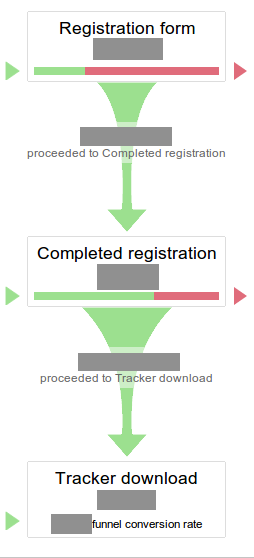
\includegraphics[width=50mm]{../images/goalfunnel}
    \end{wrapfigure}

    Bijvoorbeeld het doel van mensen aanmelden. Je kijkt dan vanaf welke pagina's mensen op het aanmeldformulier komen, en hoeveel van die mensen zich daadwerkelijk aanmelden. Het proces heet en Goal Funnel. Deze naam is gekozen omdat de gegevens vaan een trechtervorm hebben. Veel mensen komen op de homepagina, een kleiner aantal klikt door naar het formulier en een nog kleiner aantal schrijft zich daadwerkelijk in. Doel van het maken van zo'n goal funnel is om knelpunten te vinden. Zo kan er op \'e\'en bepaald punt in de rij van pagina's een probleem zitten waardoor de meeste mensen afhaken. Dit merk je omdat de trechter dan opeens v\'e\'e;l dunner wordt.

    Het doel van zo'n funnel analyseren is uitvinden op welke manier je de trechtervorm dikker kan krijgen, en dus meer mensen het door jouw gestelde doel kan laten bereiken. Doordat je op een goede manier kan laten zien waar de knelpunten zitten, kun je dit stap voor stap oplossen.

    \subsection{Bounce Rates}
    Bounce Rates is de term voor het percentage wat op een pagina komt, en niet verder klikt naar andere pagina's. Een hoge bounce rate betekent doorgaans dat de pagina niet is wat de gebruiker er van verwachte op het moment dat hij de pagina bezocht. Wanneer je weet welke pagina's een hoge bounce rate hebben, kan je onderzoeken \emph{waarom} die pagina's een hoge bounce rate hebben. Bijvoorbeeld omdat de naam van de pagina niet overeenkomt met de inhoud, of omdat de informatie op de pagina niet volledig genoeg is. Vaak is het zo dat een pagina simpelweg geen goede vervolgstap biedt, en het voor de gebruiker niet duidelijk is wat hij of zij nu moet doen.

    De belangrijkste pagina met betrekking tot Bounce Rates is doorgaans de homepagina. Dit is de pagina die nieuwe bezoekers voor het eerst zien, en de pagina die ze moet overhalen om zich aan te melden. Wanneer hier geen duidelijke vervolgstap op staat, of de gebruiker wordt niet genoeg gemotiveerd, zorgt dit voor een hogere bounce rate.

    Bij Wakoopa is de homepagina de pagina met de hoogste bounce rate, ongeveer een op de twee bezoekers klikken niet verder. Als je vervolgens kijkt waar bezoekers dan w\'el op klikken, dan is met 8\% de link naar de homepagina de hoogste. Hieruit kunnen we opmaken dat voor een percentage niet duidelijk is dat het hier om de homepagina gaat. Dit kunnen we oplossen door op de homepagina niet de link naar de homepagina te laten zien.

    Daarintegen klikt een op de vier bezoekers door naar de signup pagina, waar vervolgens meer dan de helft zich ook daadwerkelijk inschrijft (dit komt uit de signup funnel). Dat zijn hoge cijfers. Niettemin moet het lukken dit hoger te krijgen door ervoor te zorgen dat mensen op de homepagina minder snel wegklikken. Onder andere het onderzoek van \cite{Hoekman2008} doet een voorstel van hoe dit verbeterd kan worden.

    \subsection{Custom Tracking}
    Veel learning networks maken gebruik van \emph{AJAX}, een term die gebruikt wordt om aan te duiden dat delen van de pagina informatie van de server halen, maar niet de gehele pagina verversen. Het nadeel van deze techniek is dat er geen nieuwe \emph{page view} is, en dat dit dus ook niet automatisch met een statistiekprogramma wordt bijgehouden. In Google analytics heb je de mogelijkheid om via JavaScript zelf aan tracking te doen. Door een klein stukje code kan je aangeven dat iemand iets via AJAX heeft opgevraagd:
    \begin{verbatim}
    pageTracker._trackPageview(’/event/nameofevent’);
    \end{verbatim}
    Op deze manier kan je als learning network een hoop verschillende gebeurtenissen bijhouden. Bijvoorbeeld hoe vaak er op een banner wordt geklikt, of een comment wordt ingevoerd. Je krijgt hiermee inzicht in hoevaak een bepaalde functie wordt gebruikt.

    Op Wakoopa werd nog geen van de javascript opties getracked. Met behulp van van bovenstaande code is dit ingebouwd zodat we kunnen analyseren welke functies veel gebruikt worden. Ter verduidelijking zullen we een niet-bestaande boomstructuur gebruiken, in de vorm van \emph{/javascript/pagina-naam/naam-van-functie}. Door middel van de filters in Google Analytics kunnen deze dan gemakkelijk gevonden worden.

     De volgende items zullen worden getracked:
     \begin{itemize}
     \item vergroten van een screenshot
     \item bekijken van de category graph, periode dag
     \item bekijken van de category graph, periode week
     \item bekijken van de category graph, periode maand
     \item bekijken van de most used graph, periode dag
     \item bekijken van de most used graph, periode week
     \item bekijken van de most used graph, periode maand
     \item openen van de redenatie voor een aanbeveling
     \item het verwijderen van een aanbeveling
     \item het schrijven van een review
     \item zoeken via een ajax zoekveld
     \item openen van het favorite-toevoegen blok op een software pagina
     \item toevoegen van een favorite
     \item scrollen door gebruikers op een software pagina
     \item scrollen door screenshots op een software pagina
     \item openen van het tag-toevoegen blok op een software pagina
     \item toevoegen van een tag
     \item iemand toevoegen als contact
     \item verwijderen van een favorite
     \item openen van het privacy-settins blok op een software pagina
     \item verbergen van de intro promobar
     \item verzenden van een bericht via een reply
     \item verbergen van de promobar
     \item verbergen van de profile-completion bar
     \item laten zien van de software editing guidelines
     \end{itemize}



    \subsection{Heatmaps}
      \begin{figure}
      \begin{center}
      \caption{Heatmap van de homepagina}
        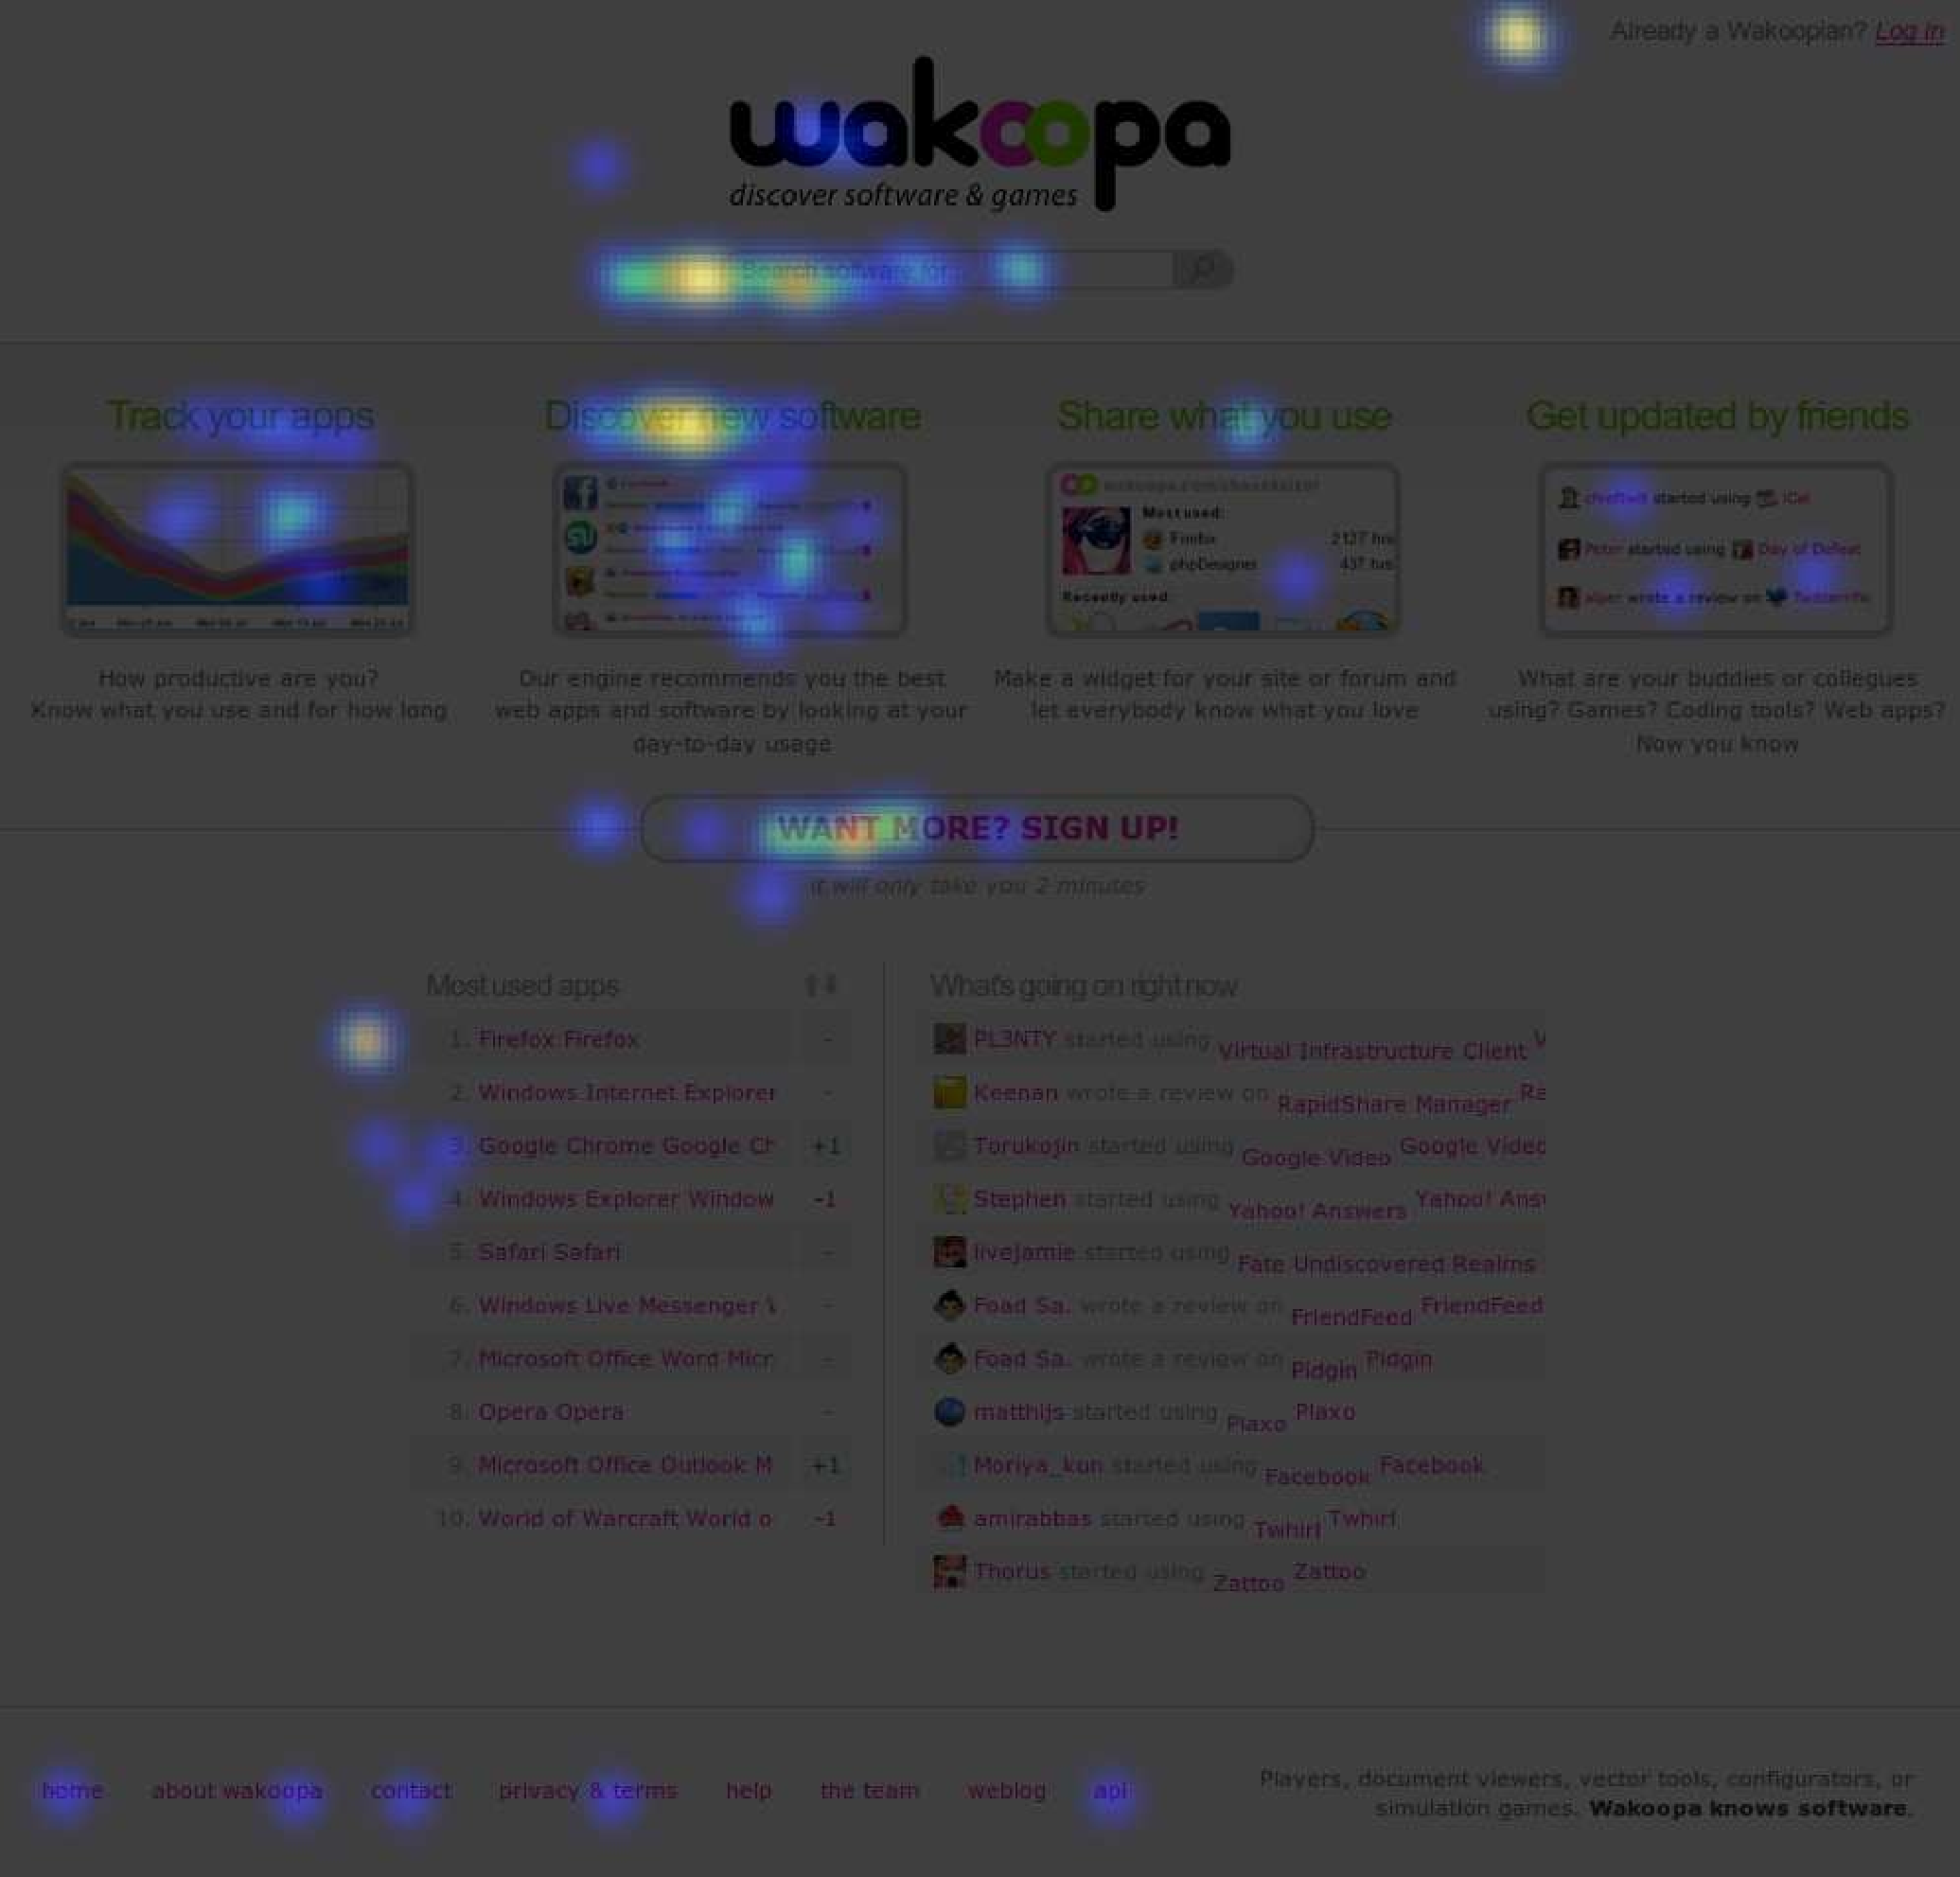
\includegraphics[width=70mm]{../images/heatmap}
      \label{heatmap}
      \end{center}
    \end{figure}
    Een techniek die pas sinds een paar jaar toegepast wordt is het maken van heatmaps. Deze heatmaps zien eruit als hittemappen, maar geven in plaats van temperatuur de hoeveelheid clicks of de positie van de muis aan op een website. Gedurende een vastgestelde periode houd je iedere click bij via javascript. Dit kan je dan later `plotten' op een screenshot, en zo zien waar het meest geklikt wordt. Omdat dit vrij intensief is voor de browser van de bezoeker, wordt het pas sinds recent toegepast, en nooit voor een lange duur.

    Door middel van deze techniek kan je goed zien welke delen van de pagina wel en welke delen niet worden gebruikt door je bezoekers. In Figuur \ref{heatmap} zie je een voorbeeld van de homepagina van Wakoopa, gemaakt met Crazyegg.\footnote{\url{http://crazyegg.com}} Wat hier opvalt is dat van de 4 afbeeldingen in het midden van de pagina, enkel de linker twee het meest worden aangeklikt. Hieruit kan je opmaken dat deze twee voor veel mensen interessanter zijn dan de rechter twee. Omgekeerd, de rechter twee zijn niet duidelijk genoeg, of wekken vergeleken met de linker twee niet even veel interesse. Een verbeterpunt. Het is dan aan de ontwikkelaar om te beslissen of dit betekent dat de rechter twee verbeterd moeten worden, weggehaald, of minder nadruk moeten krijgen waarbij de linker twee meer nadruk krijgen.

    Het is belangrijk om voordat je een heatmap laat genereren, te bepalen wat de doelen op een pagina zijn, waar de bezoeker moet klikken en welke delen welke soort bezoeker moeten aanspreken. Wanneer je dit doet is het achteraf gemakkelijk om te kijken in hoeverre bezoekers de pagina gebruiken op de manier dat jij bedoelde, en of de doelen die je hebt opgestelt ook daadwerkelijk behaald worden.


    \section{A/B testing}
    A/B testing, of multivariate testing, is een methode om twee (A/B) of meerdere (multivariate) variaties op een pagina of lay-out te testen, door deze gedurende een periode willekeurig onder bezoekers te verdelen. Bezoeker \emph{A} krijgt bijvoorbeeld variatie 1 te zien, en bezoeker \emph{B} krijgt variatie 2 te zien. Vervolgens kijk je welke gebruiker sneller of vaker op de door jouw gekozen link klikt of actie uitvoerd. Wanneer je dit met een groot aantal bezoekers gedurende een langere tijd doet, kan je hier statistische analyse op uitvoeren.

   Het ontwikkelplatform wat Wakoopa gebruikt, Ruby on Rails, heeft door middel van een plugin de optie om A/B testen uit te voeren. Deze automatiseert het verdelen van de verschillende opties tussen bezoekers en houd per variatie bij hoe vaak de geteste links of functionaliteit aangeklikt wordt.

    Naar aanleiding van de in Hoofdstuk \ref{researchchapter} genoemde onderzoeken hebben we een aantal A/B tests uitgevoerd, die hieronder beschreven staan:

    \subsection{Plaats van de sign-up link op landing pages}
      \label{ctatest}
      In tegenstelling tot de homepagina hebben onze landing pages (Pagina's waar bezoekers via zoekmachines op terecht komen) wel een sign-up link in de header. Momenteel staat deze in de linkerbovenhoek. In deze A/B test bekijken we of een variate waarin deze in de rechterbovenhoek staat, tot meer clicks leidt dan wanneer deze in de linkerbovenhoek staat. De resultaten staan in Tabel \ref{tab:signupcta}, de conclusie in Hoofdstuk \ref{wak:Editorial2008}.

        \begin{table}[ht]
        \centering
        \caption{Resultaten van de sign-up link}
        \begin{tabular}{r|*{3}{c}}
          \textbf{Versie}  & Conversie  & Verbetering & Clicks / Pageviews \\ \hline
          \textbf{Links}   & 0.00036\%  & \emph{n.v.t.}        & 1544 / 4200125 \\
          Rechts  & 0.00025\%  & -32\%                & 1058 / 4199310 \\
        \end{tabular}

        \label{tab:signupcta}
        \end{table}
    \begin{figure}
      \caption{Links}
      
\includegraphics[width=\textwidth]{../images/abtest/left}
      \caption{Rechts}
      
\includegraphics[width=\textwidth]{../images/abtest/right}
    \end{figure}

    \subsection{Het benoemen van de mate waarin een profiel is ingevuld}
      \label{profileprogress}
      Wakoopa geeft gebruikers al een berichtje na het inloggen wanneer een profiel nog niet volledig is ingevuld. Uit onderzoek van \cite{Brouns2008} blijkt dat het effectiever is om hier een vervolgstap of een progressiemeter neer te zetten. In deze test bekijken we een viertal variaties: De huidige berichtgeving, een berichtgeving met welk eerstvolgende veld ze nog moeten invullen (bv. Bio), een berichtgeving met een progressiemeter, en een berichtgeving met zowel een progressiemeter als wel eerstvolgende veld ingevuld moet worden.  De resultaten staan in Tabel \ref{tab:profilecta}, de conclusie in Hoofdstuk \ref{wak:Brouns2008}

        \begin{table}[ht]
        \centering
        \caption{Resultaten van het benoemen van de mate waarin een profiel is ingevuld}
        \rowcolors{1}{white}{lightgray}
        \begin{tabular}{r|*{3}{c}}
          \textbf{Versie}                   & Conversie  & Verbetering   & Clicks / Pageviews \\ \hline
          Origineel                         & 9\%        & \emph{n.v.t.} & 502 / 5357 \\
          Met suggestie                     & 7\%        & -22\%         & 430 / 5402\\
          \textbf{Met progressiemeter}      & 15\%       & 66\%          & 819 / 5355\\
          Met beide  & 12\%       & 33\%          & 635 / 5284\\
        \end{tabular}
        \label{tab:profilecta}
        \end{table}

    \begin{figure}
      \caption{origineel}
      
\includegraphics[width=\textwidth]{../images/abtest/original}

      \caption{met suggestie}
      
\includegraphics[width=\textwidth]{../images/abtest/suggestion}

      \caption{met progressiemeter}
      
\includegraphics[width=\textwidth]{../images/abtest/progresbar}

      \caption{met suggestie en progressiemeter}
      
\includegraphics[width=\textwidth]{../images/abtest/both}
    \end{figure}

  \newpage
  \chapter{Usabilitytechnieken die de participatie op een learning network verhogen}


  \newpage
  \chapter{Welke verbeteringen zijn er specifiek voor Wakoopa door te voeren?}
    \newpage

    Dit hoofdstuk gaat expliciet in op verbeteringen voor Wakoopa, zoals gebleken uit de vorige hoofdstukken. We passen de theorie uit hoofdstuk \ref{researchchapter}, de gebruikersonderzoeken van hoofdstuk \ref{userchapter} en de data van hoofdstuk \ref{datachapter} toe op Wakoopa en beschrijven de bevindingen en aanbevelingen.

    \section{Onderzoeken}
    Naar aanleiding van de onderzoeken in hoofdstuk \ref{researchchapter} zijn er voor Wakoopa de volgende verbeteringen:

 \subsection{\cite{Beenen2004}}
      In dit onderzoek wordt veel nadruk gelegd op de \emph{call to actions}. Deze moeten een intrinsieke motivatie stimuleren, maar er niet voor zorgen dat het lijkt alsof dit een extrinsieke motivatie is. De call to actions op de homepagina zijn een goed voorbeeld om te onderzoeken of deze inderdaad voldoen aan dit vereiste.

      \paragraph{\textbf{Verbeterpunten:}}
      \begin{itemize}
        \item Call to actions op homepagina aanpassen
      \end{itemize}

    \subsection{\cite{Berlanga2007}}
    Een aantal van de punten uit het onderzoek van \citeauthor{Berlanga2007} werden in het geval van Wakoopa al gebruikt. Het is gemakkelijk om nieuwe connecties te leggen (dit kan via een enkele klik op iemands profiel) en dit wordt gestimuleerd door aan te geven welke gebruikers op jou lijken. Gebruikers krijgen een bericht wanneer hun vrienden nieuwe applicaties gebruiken, een review schrijven, een level omhoog gaan of iets op een teampagina schrijven. De effectiviteit van dit punt wordt ook ondersteund door onderzoek van \cite{Berlanga2007}. Nieuwsgierigheid wordt gestimuleerd door het puntensysteem, waarbij gebruikers meer punten verdienen door meer software te gebruiken en door acties op de site uit te voeren. Er wordt hier enkel het level getoond, en niet het totaal aantal punten. Door dit toe voegen bied je ook voor mensen die op eht hoogste level zitten een manier om zich met anderen te vergelijken. Een ander punt waar verbetering te behalen valt is het langer vasthouden van bezoekers. Wakoopa kan dit verbeteren door mensen meer acties op de site uit te laten voeren, en interessante(re) statistieken weer te geven op profielen.

      \paragraph{\textbf{Verbeterpunten:}}
      \begin{itemize}
        \item Totaal aantal punten op het profiel laten zien
        \item Bestaande functionaliteit uitbreiden
        \item Meer statistieken bieden
      \end{itemize}


    \subsection{\cite{Brouns2008}}
    \label{wak:Brouns2008}
    Wakoopa toonde enkel een melding dat een profiel nog niet compleet was, zonder vervolgstappen aan te geven. Door het implementeren van een progressiemeter zijn er 15\% meer mensen die doorklikken naar hun accountgegevens.

    Dit resultaat bleek uit een A/B test in hoofdstuk \ref{datachapter} (zie pagina \pageref{profileprogress}). Uit deze A/B test bleek dat enkel het tonen van een progressiemeter effectiever is dan het tonen van enkel een bericht, een bericht met een suggestie van een leeg veld of het tonen van een bericht met zowel een progressiemeter en een suggestie. Mogelijke verklaringen hiervoor zijn dat de zin te lang wordt wanneer er ook een suggestie in staat, of dat de suggestie velden aangeeft die mensen niet in willen vullen.

      \paragraph{\textbf{Verbeterpunten:}}
      \begin{itemize}
        \item Toevoegen van een progressiemeter met in hoeverre het profiel is gevuld
      \end{itemize}

    \subsection{\cite{Editorial2008}}
    \label{wak:Editorial2008}
    Het merendeel van de onderzochte sociale netwerken heeft een signup call to action in de rechterbovenhoek staan. Bij Wakoopa staat deze onder het logo aan de linkerkant. Door middel van een A/B test (zie pagina \pageref{ctatest}) is gekeken of dit ook voor Wakoopa meer clicks opleverde. Opvallend genoeg bleek rechts ongeveer twee keer zo slecht te werken als links. Hier zijn twee mogelijke verklaringen voor. De eerste is dat de call to action links al direct onder het logo stond, een plek waar veel mensen bij het openen van een nieuwe site als eerste kijken\footnote{\url{http://www.useit.com/alertbox/reading\_pattern.html}}. Een andere verklaring is \emph{banner blindness}. Omdat de call to action rechts naast de banner stond en het leek alsof de call to action daarbij hoorde, zullen mensen eerst de banner zien en dan automatisch de banner negeren, en daarmee ook de call to action negeren.\footnote{\url{http://www.useit.com/alertbox/fancy-formatting.html}}

      \paragraph{\textbf{Verbeterpunten:}}
      \begin{itemize}
        \item Geen
      \end{itemize}

    \subsection{\cite{Wroblewski2009}}
    Wakoopa past bij het aanmelden van een nieuwe account al de meest effectieve vorm van inline validatie toe, maar op andere plekken wordt dit nog niet gedaan. Op de account pagina kan inline validatie goed worden toegepast, om aan te geven of een nieuw wachtwoord goed genoeg is, of een wachtwoord en het controlewachtwoord overeenkomen en om aan te geven en of het ingevoerde emailadres voldoet.

      \paragraph{\textbf{Verbeterpunten:}}
      \begin{itemize}
        \item Validatie toevoegen aan de account settings pagina
      \end{itemize}

    \subsection{\cite{Alfrink2008}}
    Sinds dit rapport heeft Wakoopa een speciale pagina aangemaakt die de gebruiker direct ziet na het aanmelden, waar in punten uit wordt gelegd welke vervolgstappen een nieuwe gebruiker heeft (de tracker downloaden, contacten zoeken, naar zijn dashboard gaan). Op andere punten kan Wakoopa dit beter stimuleren, bijvoorbeeld door middel van e-mails wanneer een gebruiker een week of twee weken lang de service niet heeft gebruikt, of alerts wanneer een gebruiker een applicatie veel gebruikt maar nog niet heeft gereviewt. Deze twee directe vragen om participatie zouden volgens \citeauthor{Alfrink2008} zeer geschikt zijn om in te zetten.

    Naast deze oproepen tot participatie noemt \citeauthor{Alfrink2008} het weergeven van persoonlijke informatie op algemene pagina's als een punt van verbetering. Sinds dit rapport wordt er al veel persoonlijke informatie weergegeven op bijvoorbeeld de software en developer-pagina's, maar niet op bijvoorbeeld de categoriepagina's, waar je heel goed een top-5 van door jouw gebruikte applicaties in die categorie kan laten zien.
    \paragraph{\textbf{Verbeterpunten:}}
      \begin{itemize}
        \item Alerts geven wanneer een gebruiker een applicatie langer dan vijf uur gebruikt heeft maar nog geen review heeft geschreven
        \item E-mail sturen wanneer een gebruiker twee weken geen software heeft getrackt.
        \item Een persoonlijke top 5 toevoegen op de categoriepagina's
      \end{itemize}

    \subsection{\cite{Hoekman2008}}
    Het grootste kritiekpunt uit dit onderzoek was de navigatie en de indeling van de homepagina. De homepagina had niet \'e\'en duidelijk focuspunt en de vier punten geven niet duidelijk genoeg de voordelen van Wakoopa weer. Voor de navigatie stellen ze voor om deze te herstructureren naar drie niveau's, gefocust op gebruikersdoelen. Hoewel dit niet in het onderzoek wordt genoemd, kunnen we dit goed doen door middel van het maken van persona's en vanuit deze persona's een cardsorting sessie te houden.

    Naast deze twee punten noemde Hoekman de inconsistentie van kleurgecodeerde gebieden op de site. Een specifiek probleempunt is dat sommige mededelingen in eenzelfde soort geel als de persoonlijke punten worden weergegeven, deze kleur kan beter in een neutrale kleur worden omgezet.

    \paragraph{\textbf{Verbeterpunten:}}
      \begin{itemize}
        \item Navigatiestructuur focussen op gebruikersdoelen
        \item Homepagina re-align maken, waarin de aandacht gaat naar voordelen in een duidelijk blok, en er meer uitleg is.
        \item De kleur van mededelingen veranderen in een neutralere kleur.
      \end{itemize}

    \subsection{\cite{Timmerman2008}}
    In dit onderzoek wordt veel verwezen naar het analyseren van data en gebruik van andere usabilitytechnieken dan een expert review. Het analyseren van Statistieken, het gebruik van A/B testen en het maken van persona's worden als nuttige middelen genoemt. Door middel van deze persona's kan bij (nieuwe) functionaliteit worden gekeken of dit wel overeenkomt met gebruikersdoelen.

    \paragraph{\textbf{Verbeterpunten:}}
      \begin{itemize}
        \item Maak persona's en gebruikersdoelen
        \item Analyseer de statistieken op trends
      \end{itemize}


  \newpage
  \chapter{De quick wins om participatie te verhogen op learning networks}
    \newpage

  \newpage
  \chapter*{Conclusie en Aanbevelingen}
  \addcontentsline{toc}{chapter}{Conclusie en Aanbevelingen}

  \newpage
  \chapter*{Discussie}
  \addcontentsline{toc}{chapter}{Discussie}

  \newpage
  \chapter*{Verklarende woordenlijst}
  \addcontentsline{toc}{chapter}{Verklarende woordenlijst}

  \listoftables
  \addcontentsline{toc}{chapter}{Lijst van tabellen}

  \newpage
  \bibliography{../references/referenties}
  \bibliographystyle{plainnat}
  \addcontentsline{toc}{chapter}{Bibliografie}
\end{document}

